\documentclass[10pt,a4paper]{article}
\usepackage{amsmath,amssymb,amsthm,graphicx}
\newcommand{\Sel}{\operatorname{Sel}}
\newcommand{\Sort}{\operatorname{Sort}}
\newcommand{\uSel}{\widetilde{\operatorname{Sel}}}
\newcommand{\calS}{\mathcal S}
\newcommand{\bits}{\{0,1\}}
\newcommand{\ZZ}{\mathbb Z}
\newcommand{\NN}{\mathbb N}
\newenvironment{originalresult}[1]{\par\medskip\noindent\textbf{#1.}\itshape}{\par\medskip}
\title{Linear-size logarithmic-depth Boolean circuits for multiselection}
\author{Justin Holmgren, Ron Rothblum}
\date{doi:10.4230/LIPIcs.CCC.2024.11; CC BY 4.0}
\begin{document}
\maketitle
\noindent\textit{Editorial note.} Faithful editable TeX transcription of the official CC BY4.0 published PDF, including Sections3-7 and all source-local supporting proofs. Figure1 is included from the original PDF only as a cropped figure; mathematical body is editable text. Original source notation/dimensions and wording retained. Native TeX was not located. Standard cited prior constructions are exact prerequisites, not recursively reproved. No author mathematics is supplemented; applications and the separate uniformity extension are outside this main-result material.\par\medskip
\noindent\textit{Allowed standard prerequisites (editorial).}\begin{itemize}
\item AKS sorting networks. Ajtai, Komlos and Szemeredi [1], source Lemma8, exact invoked statement retained
\item Pippenger self-routing superconcentrator. Pippenger [25], source Theorem18, complete routing interface and author circuit simulation retained
\item Parallel prefix for associative operations. Ladner and Fischer [20], exact invoked statement retained in Lemma26 proof
\end{itemize}\medskip
\section*{Multiselection (author source pp.11:1--11:2)}
In the selection problem, also commonly called multiplexing, one is given a long string $x\in\bits^n$ and an index $i\in[n]$, and the goal is to output $x_i$. Selection is one of the basic operations in the word RAM model (and indeed costs unit time in that model). Implementing it by a Boolean circuit however is more involved and requires a circuit of size $\Theta(n)$.
In this work we investigate a natural generalization of selection, which we call multiselection; now rather than a single index, one is given indices $i_1,\ldots,i_q\in[n]$, and the goal is to compute $(x_{i_1},\ldots,x_{i_q})$. We denote this function by $\Sel^{n\to q}$. Multiselection is trivial in the word RAM model of computation (it costs $\Theta(q)$ operations with any standard instruction set). We focus on implementing multiselection by small Boolean circuits, where here and throughout this work all circuits have bounded fan-in. In this setting, we do not have matching upper and lower bounds. The best circuit size lower bound for multiselection is the input length $n+q\cdot\log n$. On the other hand, the straightforward construction (which selects each index separately) is much larger, with size $\Theta(n\cdot q)$. A slightly more sophisticated approach reduces to sorting, and results in a circuit of size $\Theta(n\log^2n)$ for any $q=O(n)$. Somewhat surprisingly, it appears that multiselection has not been systematically studied and in particular we are not aware of essentially any other upper bounds (see further discussion in Section 1.1).

\section*{3 Preliminaries (author source p.11:5)}
We assume that the reader is familiar with the notion of a Boolean circuit and the associated function that it computes. We emphasize that, unless otherwise stated, throughout this work by ``circuit'' we refer to constant fan-in circuits over the standard De Morgan base.
\subsection*{3.1 Uniformity}
We say that a family $\mathcal C=\{C_n\}_{n\in\ZZ^+}$ of Boolean circuits is log-space uniform if there exists a Turing machine that on input $1^n$ uses $O(\log n)$ space and prints the description of the circuit $C_n$, on a write-only output tape. The description is a listing of the gates in an (arbitrary) topological ordering along with a specification of the gate operation and pointers to each of its inputs. In Appendix B we also discuss an extension of our main result for linear-time uniformity.
\subsection*{3.2 Boolean Circuits for Uniselection}
The following standard proposition gives a linear-size circuit, that given a string $x\in\Sigma^n$, over an alphabet $\Sigma$, and an index $i\in[n]$, outputs the symbol $x_i$ (in other words, a multiplexer).
\begin{originalresult}{Proposition 2}
Let $s=s(n)\in\ZZ^+$ and let $\Sigma=\bits^s$. There exists a log-space uniform Boolean circuit for $\Sel_\Sigma^{n\to1}$ with size $O(n\cdot s)$ and depth $O(\log n)$.
\end{originalresult}
\begin{proof}
Without loss of generality assume that $s=1$ (for $s>1$ we can use $s$ parallel copies of the circuit for $s=1$). The circuit follows a divide and conquer strategy. Assume for simplicity that $n$ is a power of 2. Let $x\in\bits^n$ and $i\in[n]$ be the inputs. Let $i_1$ denote the most significant bit of $i$ and let $i'$ denote the remaining bits (i.e., $i'\in[n/2]$). To select the $i$th bit of $x$, the circuit recursively selects the $(i')$th bit of both the lower and upper halves of $x$. Then, based on $i_1$, it decides which of the two bits to output. Overall the circuit size satisfies the recursion: $S(n)=2S(n/2)+O(1)$ and the depth satisfies $D(n)=D(n/2)+O(1)$. The proposition follows.
\end{proof}
\subsection*{3.3 Small-Size Sorting Circuits}
Our circuits for multiselection heavily rely on circuits for sorting integers.
\begin{originalresult}{Lemma 3}
For every $k=k(n)$ and $m=m(n)$, there is a log-space uniform Boolean circuit of size $O(n\cdot m\cdot\log n)$ for sorting $n$ integers of $m$ bits.
\end{originalresult}
This lemma follows immediately from the sorting networks of Ajtai, Koml\'os, and Szemer\'edi [1]. In order to make our multiselection circuit have logarithmic depth, we need a refined version of Lemma 3, which we present in Section 4.

\section*{4 Low-Depth Sorting of Logarithmic-Length Keys (author source pp.11:5--11:9)}
We first recall what it means to sort with respect to a partial ordering.
\begin{originalresult}{Definition 4}
Let $\Sigma$ be a finite set. We say that $x,y\in\Sigma^n$ are reorderings of each other if for some permutation $\pi:[n]\to[n]$, it holds that $x_i=y_{\pi(i)}$, for all $i\in[n]$.
\end{originalresult}
\begin{originalresult}{Definition 5}
Let $\Sigma$ be a finite set with a strict partial ordering $\prec$. A Boolean circuit is said to sort $\Sigma^n$ with respect to $\prec$ if on any input $x\in\Sigma^n$, it outputs a reordering $y$ of $x$ such that for any $i,j\in[n]$, $y_i\prec y_j\implies i<j$.
\end{originalresult}
In particular, we will focus on a partial ordering that compares integers by their $k$ most significant bits. That is, for any $m\in\ZZ^+$ and any $x,y\in\bits^m$, we write $x\prec_k y$ to denote that $(x_1,\ldots,x_k)$ lexicographically precedes $(y_1,\ldots,y_k)$.
\begin{originalresult}{Lemma 6}
For every $m=m(n)$ and $k\in[m]$, there is a log-space uniform Boolean circuit of size $O(n\cdot m\cdot\log n)$ and depth $O(k+\log n)$ for sorting $(\bits^m)^n$ with respect to $\prec_k$.
\end{originalresult}
We are mainly interested in the setting $k=\Theta(\log n)$, in which case the constructed Boolean circuit has size $O(n\cdot m\cdot\log n)$ and depth $O(\log n)$.
To the best of our knowledge Lemma 6 was not previously known. The straight-forward circuit based on AKS networks yields circuits with matching size $O(n\cdot m\cdot\log n)$ but depth $O(\log n\cdot\log k)$. Kospanov [17] obtained circuits with better depth $O(\log n+\log k)$ but much larger size $O(n^2\cdot k)$. A recent work of [18] obtains size $O(n\cdot k^2)$ and depth $O(\log n+k\log k)$, which is better for some values of $k=o(\log n)$, but worse in our regime of $k=\Theta(\log n)$. The work of Lin and Shi [22, Theorem 1.1] similarly constructs circuits with size $O(n\cdot m\cdot\log n)$ and depth $O(\log n)$ when $n>2^{4k+7}$, but not for all values of $k=\Theta(\log n)$.
\subsection*{4.1 Sorting Networks}
Our sorting circuits rely on sorting networks, which are generic constructions of $n$-input sorting circuits from 2-input sorting circuits.
\begin{originalresult}{Definition 7 (Sorting Networks)}
An $n$-input sorting network is a circuit $C$ with $n$ inputs and $n$ outputs, and with all gates having fan-in and fan-out two, such that for any set $\Sigma$ with strict partial ordering $\prec$, if each gate of $C$ is replaced by a circuit that sorts $\Sigma^2$ with respect to $\prec$, then the resulting circuit sorts $\Sigma^n$ with respect to $\prec$.
\end{originalresult}
For the best asymptotic size and depth, we use the celebrated sorting network of Ajtai, Koml\'os, and Szemer\'edi [1].
\begin{originalresult}{Lemma 8 ([1])}
There is a (log-space uniform) $n$-input sorting network with size $O(n\log n)$ and depth $O(\log n)$.
\end{originalresult}
\subsection*{4.2 From Sorting Networks to Boolean Circuits}
We prove Lemma 6 by combining the following lemma with Lemma 8.
\begin{originalresult}{Lemma 9}
Suppose that there is a log-space uniform sorting network on $n$ elements with size $S=S(n)$ and depth $D=D(n)$. Then, for all $m=m(n)$ and $k\in[m]$, there is a log-space uniform Boolean circuit with size $O(S\cdot m)$ and depth $O(D+k)$ for sorting $(\bits^m)^n$ with respect to $\prec_k$.
\end{originalresult}
\begin{proof}
Starting with an $n$-input sorting network $A$ with size $S$ and depth $D$, we obtain a Boolean circuit $C$ from $A$ by replacing each gate with a Boolean circuit $\Sort^{(2)}_{k,m}$ that sorts $(\bits^m)^2$ with respect to $\prec_k$. With this approach it is easy to make $C$ have size $O(S\cdot m)$---since $\Sort^{(2)}_{k,m}$ merely needs to have size $O(m)$.
Depth seems to pose more of a difficulty. Locality considerations imply that $\Sort^{(2)}_{k,m}$ must have depth at least $\Omega(\log k)$ (e.g. the least significant bit of either output of $\Sort^{(2)}_{k,m}(x,y)$ depends on all of the $k$ most significant bits of $x$ and $y$). Thus, it might seem that this approach dooms $C$ to have depth $\Omega(D\cdot\log k)$.
We circumvent this difficulty by noting that although input-to-output paths in $C$ are concatenations of $D$ input-to-output paths in $\Sort^{(2)}_{k,m}$, these $D$ paths cannot all be worst-case. In particular, the $i$th output bit of one copy of $\Sort^{(2)}_{k,m}$ is only connected to the $j$th input bit of another copy if $i\equiv j\pmod m$ (see Figure 1).
\begin{figure}[ht]\centering\includegraphics[page=7,width=.8\textwidth,trim=90 550 105 160,clip]{multiselection-original.pdf}\caption{Original Figure 1: The four different ways that we can connect one copy of $\Sort^{(2)}_{k,n}$ to another. In this depiction, a copy of $\Sort^{(2)}_{k,n}$ is depicted by a rectangle, with inputs incident to the bottom edge and output incident to the top. The left half corresponds to the first input/output, and the right half to the second.}\end{figure}
We leverage this with the following lemma, whose proof we defer momentarily.
\begin{originalresult}{Lemma 10}
For any $m=m(n)$ and $k\in[m]$, there is a log-space uniform Boolean circuit $\Sort^{(2)}_{k,m}$ with size $O(m)$ that sorts $(\bits^m)^2$ with respect to $\prec_k$ and has the following additional property:
For all $\hat i,\hat j\in[m]$ and $i,j\in[2m]$ with $i\equiv\hat i\pmod m$ and $j\equiv\hat j\pmod m$, every path in $\Sort^{(2)}_{k,m}$ from the $i$th input vertex to the $j$th output vertex has length $O(\min(j,k)-\min(i,k)+1)$. In particular there is no such path if $k>i>j$.
\end{originalresult}
Assuming Lemma 10, consider any input-to-output path $p$ in $C$. We write $p$ as a composition of paths $p_1\circ\cdots\circ p_D$, where each $p_\ell$ is an input-to-output path of some copy of $\Sort^{(2)}_{k,m}$. Define $i_\ell,j_\ell\in[2m]$ so that $p_\ell$ starts at the $i_\ell$th input and ends at the $j_\ell$th output of that copy, and define $\hat i_\ell,\hat j_\ell\in[m]$ such that $i_\ell\equiv\hat i_\ell\pmod m$ and $j_\ell\equiv\hat j_\ell\pmod m$. By the observation above, we have $\hat j_\ell=\hat i_{\ell+1}$ for all $\ell\in[D-1]$, and by Lemma 10, we have for some constant $L$ that $|p_\ell|\le L\cdot(\min(\hat j_\ell,k)-\min(\hat i_\ell,k)+1)$.
Putting this together, we bound
\begin{align*}
|p|&=\sum_{\ell=1}^D|p_\ell|\\
&\le\sum_{\ell=1}^D L\cdot(\min(\hat j_\ell,k)-\min(\hat i_\ell,k)+1)\\
&=L\cdot(\min(\hat j_D,k)-\min(\hat i_1,k)+D)\quad\text{(telescoping sum because $\hat j_\ell=\hat i_{\ell+1}$)}\\
&\le L\cdot(k+D)=O(k+D).
\end{align*}
\end{proof}
It remains to prove Lemma 10.
\begin{proof}[Proof of Lemma 10]
We use the straightforward construction that compares the elements bit-by-bit starting with their most significant bits. In more detail, we will construct a circuit $\widetilde{\Sort}^{(2)}_{k,m}:\{\prec,?,\succ\}\times\bits^m\times\bits^m$ that has the functionality
\begin{align*}
\widetilde{\Sort}^{(2)}_{k,m}(?,x,y)&=\begin{cases}(x,y)&\text{if }x\prec y,\\(y,x)&\text{otherwise},\end{cases}\\
\widetilde{\Sort}^{(2)}_{k,m}(\prec,x,y)&=(x,y),\\
\widetilde{\Sort}^{(2)}_{k,m}(\succ,x,y)&=(y,x)
\end{align*}
and we define $\Sort^{(2)}_{k,m}=\widetilde{\Sort}^{(2)}_{k,m}(?,\cdot,\cdot)$. This clearly gives the desired functionality. The first input symbol aids in recursively constructing the circuit for $\widetilde{\Sort}^{(2)}_{k,m}$, and is meant to indicate whether the global decision on the comparison between $x$ and $y$ is (1) still undecided (?), (2) decided toward $x$ or (3) decided toward $y$.
Our construction of $\widetilde{\Sort}^{(2)}_{k,m}$ is recursive. If $k=0$, then we define $\widetilde{\Sort}^{(2)}_{k,m}$ to be the identity function. For $k>0$, $\widetilde{\Sort}^{(2)}_{k,m}$ takes input $(c,x,y)$, it first computes
\[(c',a_1,b_1)=\begin{cases}(\prec,x_1,y_1)&\text{if }c=\prec\text{ or }(c=?\text{ and }x_1<y_1),\\(?,x_1,y_1)&\text{if }c=?\text{ and }x_1=y_1,\\(\succ,y_1,x_1)&\text{if }c=\succ\text{ or }(c=?\text{ and }x_1>y_1).\end{cases}\]
Then, with $x'$ and $y'$ denoting $(x_2,\ldots,x_m)$ and $(y_2,\ldots,y_m)$, it computes
\[(a',b')=\widetilde{\Sort}^{(2)}_{k-1,m-1}(c',x',y').\]
Finally it outputs $a_1\circ a',b_1\circ b')$, where $\circ$ denotes string concatenation. It is easy to check the correctness of this construction.
\paragraph{Circuit Size.} Let $S(k,m)$ denote the size of $\widetilde{\Sort}^{(2)}_{k,m}$. For $k=0$ we clearly have $S(k,m)=O(m)$. For larger $k$, the recursive construction gives $S(k,m)=S(k-1,m-1)+O(1)$, so by induction $S(k,m)=O(m)$ for all $k\le m$.
\paragraph{Input-to-Output Path Lengths.} We now bound the length of different input-to-output paths in $\widetilde{\Sort}^{(2)}_{k,m}$. As in the construction above, denote the input to $\widetilde{\Sort}^{(2)}_{k,m}$ by $(c,x,y)$ and denote the output by $(a,b)$.
\begin{originalresult}{Claim 11}
There exists a constant $L$ such that any path in $\widetilde{\Sort}^{(2)}_{k,m}$ from an input $\{x_i,y_i\}$ to an output $\{a_j,b_j\}$ has length at most $L\cdot(j-i+1)$, and any path from the input $c$ to an output $\{a_j,b_j\}$ has length at most $L\cdot j$. In particular any path to an output $\{a_j,b_j\}$ has length at most $L\cdot j$.
\end{originalresult}
\begin{proof}
Let $(x',y')$ denote the input to the recursive call to $\widetilde{\Sort}^{(2)}_{k-1,m-1}$ and let $(a',b')$ denote the output of this call. We consider several cases separately:
\begin{itemize}
\item Paths to $\{a_1,b_1\}$ have length bounded by an absolute constant because $a_1$ and $b_1$ are just a (constant-sized) function of the inputs $(c,x_1,y_1)$. If $L$ is sufficiently large then this constant is at most $L$.
\item For $j>1$, paths from $\{c,x_1,y_1\}$ to $a_j$ $(=a'_{j-1})$ consist of a path through a constant-sized circuit (the computation of $c'$) concatenated with a path to $a'_{j-1}$ in $\widetilde{\Sort}^{(2)}_{k-1,m-1}$. By induction the latter path has length at most $L\cdot(j-1)$, so if $L$ is sufficiently large then the total path length is at most $L\cdot j$.
\item For $i>1$ and $j>1$, paths from $\{x_i,y_i\}$ to $\{a_j,b_j\}$ are just paths from $\{x'_{i-1},y'_{i-1}\}$ to $\{a'_{j-1},b'_{j-1}\}$ and thus by induction they have length at most $L\cdot(j-i+1)$.
\end{itemize}
\end{proof}
Returning to $\Sort^{(2)}_{k,m}=\widetilde{\Sort}^{(2)}_{k,m}(?,\cdot,\cdot)$ (without the tilde), we can see that any input-to-output path in $\Sort^{(2)}_{k,m}$ directly corresponds to an input-to-output path in $\widetilde{\Sort}^{(2)}_{k,m}$ whose length is appropriately bounded by Claim 11. That concludes the proof of Lemma 10.
\end{proof}

\section*{5 Unordered Multiselection Over Large Alphabets (author source pp.11:9--11:13)}
In this section we construct a circuit that implements a relaxation of multiselection. Informally, this relaxation allows the output elements to appear in any order (and possibly with repetitions), rather than the same order in which they were queried. Additionally, rather than selecting individual bits (which is our eventual goal)---we consider a generalization to a larger alphabet size.
\begin{originalresult}{Definition 12}
Unordered multiselection (with $q$ queries, over alphabet $\Sigma$) is the search problem defined by the relation
\[\uSel_\Sigma^{n\to q}\stackrel{\rm def}=\{((x,i),y)\in(\Sigma^n\times[n]^q)\times(\Sigma\cup\{\bot\})^q:\{y_k:y_k\ne\bot\}_{k\in[q]}=\{x_{i_k}\}_{k\in[q]}\}.\]
\end{originalresult}
\subsection*{5.1 Superconcentrators and Routing}
We recall the notion of a superconcentrator, which is the main technical tool involved in our construction of Boolean circuits for unordered multiselection.
\begin{originalresult}{Definition 13 (Networks)}
A network $N$ is a tuple $N=(V,E,A,B)$, where $G=(V,E)$ is a directed acyclic graph and $A,B\subseteq V$ are respectively sets of sources and sinks in $G$.
If $|A|=|B|=n$, then $N$ is said to be an $n$-network. The size of $N$, denoted by $|N|$, is defined to be $|E|$; the degree of $N$ is the degree of $G$; and the depth of $N$ is the longest path length in $G$.
A family of $n$-networks $\{N_n\}_{n\in\ZZ^+}$ is said to be log-space uniform if there an algorithm that on input $1^n$ runs in $O(\log n)$ space and outputs $G$ (say with an adjacency list representation) and $A,B$ (say represented by indicator strings).
\end{originalresult}
\begin{originalresult}{Definition 14 (Superconcentrators)}
An $n$-network $N=(V,E,A,B)$ is said to be a superconcentrator if for all $q\in[n]$ and all subsets $X\subseteq A$ and $Y\subseteq B$ with $|X|=|Y|=q$, there exist $q$ vertex-disjoint paths from $X$ to $Y$.
\end{originalresult}
\begin{originalresult}{Definition 15}
Let $S=(V,E,A,B)$ be an $n$-superconcentrator. The routing problem for $S$ is a search problem $\operatorname{Route}_S$ whose input is a pair of (indicator strings for) sets $X\subseteq A,Y\subseteq B$ with $|X|=|Y|$. A valid corresponding output is any (indicator string for a) set $R\subseteq E$ of edges such that $R$ is a union of $q$ vertex-disjoint paths from $X$ to $Y$, where $q=|X|=|Y|$.
\end{originalresult}
Note that whenever $S$ is an $n$-superconcentrator, the search problem $\operatorname{Route}_S$ is total. Naturally, it is desirable for a superconcentrator $S$ to admit efficient algorithms for $\operatorname{Route}_S$. The state of the art in this respect is Pippenger's construction of a ``self-routing'' superconcentrator.
Informally, a delay-$d$ self-routing protocol for a superconcentrator $(V,E,A,B)$ associates each vertex $v\in V$ with a finite automaton that can communicate synchronously with the automata on neighboring vertices (where $u$ is said to neighbor $v$ if $(u,v)$ or $(v,u)$ is in $E$). For any sets $X\subseteq A$ and $Y\subseteq B$ with $|X|=|Y|=q$, if the automata in $X$ and $Y$ are initialized with state 1, and all other automata are initialized with state 0, then in $d$ steps the automata jointly compute $q$ vertex-disjoint paths from $X$ to $Y$ by on the $d$th step transmitting 1 on all edges in those paths and 0 on other edges.
\begin{originalresult}{Definition 16}
A self-routing protocol with delay $d$ for an $n$-superconcentrator $S=(V,E,A,B)$ is a tuple $(\Sigma,\delta)$, where:
\begin{itemize}
\item $\Sigma$ is a finite ``alphabet'' set that contains $\{0,1\}$; and
\item $\delta:\Sigma^{V\cup E}\to\Sigma^{V\cup E}$ is a function such that:
\begin{itemize}
\item for every vertex $v\in V$ with incident edges $E_v$, $\delta(q)_v$ depends as a function of $q$ only on $(q_e)_{e\in E_v}$.
\item for every edge $e=(u,v)\in E$, $\delta(q)_e$ depends as a function of $q$ only on $q_u$ and $q_v$.
\end{itemize}
\end{itemize}
For any sets $X\subseteq A$ and $Y\subseteq B$ with $|X|=|Y|$, if we define $q^{(0)}\in\Sigma^{V\cup E}$ by
\[q_v^{(0)}\stackrel{\rm def}=\begin{cases}1&\text{if }v\in X\cup Y,\\0&\text{if }v\in V\setminus(X\cup Y),\end{cases}\]
and $q_e^{(0)}\stackrel{\rm def}=0$ for all $e\in E$, then the set
\[R\stackrel{\rm def}=\{e\in E:\delta^d(q^{(0)})_e=1\}\]
satisfies $((1_X,1_Y),1_R)\in\operatorname{Route}_S$.
Such a self-routing protocol for an $n$-superconcentrator is said to be log-space uniform if there is a log-space Turing machine that on input $1^n$ outputs:
\begin{itemize}
\item a description of $\Sigma$;
\item for each $v\in V$ with incident edges $E_v$, the truth table for $\delta(q)_v$ as a function of $(q_e)_{e\in E_v}$.
\item for each $e=(u,v)\in E$, the truth table for $\delta(q)_e$ as a function of $(q_u,q_v)$.
\end{itemize}
\end{originalresult}
\begin{originalresult}{Definition 17}
A self-routing superconcentrator is a superconcentrator $S$ with an associated self-routing protocol $(\Sigma,\delta)$ for $S$. A self-routing superconcentrator is said to be log-space uniform if both the superconcentrator and the associated self-routing protocol are log-space uniform.
\end{originalresult}
\begin{originalresult}{Theorem 18 ([25])}
There exists a log-space uniform self-routing $n$-superconcentrator $S$ with size $O(n)$, degree $O(1)$, and depth $O(\log n)$, where the self-routing protocol has alphabet size $O(1)$ and delay $O(\log n)$.
\end{originalresult}
\begin{originalresult}{Corollary 19}
There exists a log-space uniform $n$-superconcentrator $S$ with size $O(n)$, degree $O(1)$, and depth $O(\log n)$, such that $\operatorname{Route}_S$ is solvable by a log-space uniform Boolean circuit of size $O(n\log n)$ and depth $O(\log n)$.
\end{originalresult}
\begin{proof}
Let $S=(V,E,A,B)$ be the log-space uniform self-routing superconcentrator given by Theorem 18, let the self-routing protocol be given by $(\Sigma,\delta)$, and let $d=O(\log n)$ denote the delay of this self-routing protocol. To prove the corollary, we need to construct a log-space uniform Boolean circuit for solving $\operatorname{Route}_S$, with size $O(n\log n)$ and depth $O(\log n)$.
We are given $1_X$ and $1_Y$. The circuit starts by computing $q^{(0)}\in\Sigma^{V\cup E}$ as defined in Definition 16. By construction this can be done with a circuitry of size $O(n)$ and depth $O(1)$. The circuit next computes $\delta^d(q^{(0)})$. Recall that each output symbol of $\delta(q)$ depends on at most $\deg(S)=O(1)$ symbols of $q$. Since the alphabet $\Sigma$ is also constant-sized, this means that $\delta$ is implementable by a (log-space uniform) circuit of size $O(|V\cup E|)=O(n)$ and depth $O(1)$. Iterating this circuit $d$ times, we compute $\delta^d(q^{(0)})$ with log-space uniform circuitry of size $O(d\cdot n)$ and depth $O(d)$. Finally, we extract from $\delta^d(q^{(0)})$ the indicator string $1_R$ for the set
\[R\stackrel{\rm def}=\{e\in E:\delta^d(q^{(0)})_e=1\}.\]
This takes (log-space uniform) circuitry of size $O(|E|)=O(n)$ and depth $O(1)$.
In total, this circuit for computing $1_R$ is log-space uniform and has size $O(n\cdot d)=O(n\log n)$ and depth $O(d)=O(\log n)$. By the definition of a self-routing protocol, $R$ satisfies $((1_X,1_Y),1_R)\in\operatorname{Route}_S$, i.e. the circuit solves $\operatorname{Route}_S$.
\end{proof}
\subsection*{5.2 From Superconcentrators To Unordered Multiselection}
\begin{originalresult}{Proposition 20}
Let $n\in\ZZ^+$, let $s=s(n)$ satisfy $s=\Omega(\log^2n)$, and let $\Sigma=\bits^s$. For any $q=q(n)\in[n]$ there exists a log-space uniform Boolean circuit for $\uSel_\Sigma^{n\to q}$ with size $O(n\cdot s)$ and depth $O(\log n)$.
\end{originalresult}
\begin{proof}
Let $S=(V,E,A,B)$ be a log-space uniform $n$-superconcentrator with size $O(n)$, depth $O(\log n)$, degree $O(1)$ such that $\operatorname{Route}_S$ is solvable by a log-space uniform Boolean circuit of size $O(n\log n)$ and depth $O(\log n)$. (Such an $S$ is guaranteed to exist by Corollary 19). Order the elements of $A$ and $B$ arbitrarily so that $A=\{a_1,\ldots,a_n\}$ and $B=\{b_1,\ldots,b_n\}$.
\paragraph{The Circuit.} Our circuit, taking as input $x\in\Sigma^n$ and $(i_1,\ldots,i_q)\in[n]^q$, is constructed in two parts.
The first part of our circuit computes indicator strings $1_X\in\bits^A$, $1_Y\in\bits^B$, and $1_R\in\bits^E$ for sets $X\subseteq A,Y\subseteq B$, and $R\subseteq E$ defined as follows. The set $X$ is defined as $\{a_{i_1},\ldots,a_{i_q}\}$, $Y$ is defined as $\{b_1,\ldots,b_{q'}\}$, where $q'$ is the cardinality of $X$ (which may be smaller than $q$ due to repetitions), and $R$ is the edges of $q'$ vertex-disjoint paths from $X$ to $Y$.
The second part of our circuit consists of a gadget $g_v$ for each vertex $v\in V$. For a vertex $v\in A$, say $v=a_j$, the gadget $g_v$ simply outputs $x_j$ if $v\in X$ and $\bot$ otherwise. For other $v$, i.e. with positive in-degree $d$, the gadget $g_v$ is a circuit for $\Sel_{\Sigma\cup\{\bot\}}^{d\to1}$ (e.g. the circuit from Proposition 2). To construct the inputs for $g_v$, first order the in-neighbors of $v$ arbitrarily as $u_1,\ldots,u_d$. The data input for $g_v$ is then constructed by taking the $i$th symbol, for any $i\in[d]$, to be the output of $g_{u_i}$. The selector input for $g_v$ is constructed to be (the unique) $i^\star\in[d]$ such that $(u_{i^\star},v)\in R$ if such an $i^\star$ exists, and arbitrary otherwise.
Finally, the outputs of our circuit are the outputs of $g_{b_1},\ldots,g_{b_q}$.
\paragraph{Size and Depth.} In the first part of our circuit, the computation of $1_X$ uses log-space uniform circuitry of size $O(n\log^2n)=O(n\cdot s)$ and depth $O(\log n)$ by Lemma 21 below. Next, $1_Y$ is obtained by sorting $1_X$ with log-space uniform circuitry of size $O(n\log n)$ and depth $O(\log n)$ (this is possible by Lemma 8). Finally, the computation of $1_R$ uses log-space uniform circuitry of size $O(n\log n)$ and depth $O(\log n)$ because of our choice of superconcentrator $S$. In total the circuitry of this part has size $O(n\cdot s)$ and depth $O(\log n)$.
In the second part of our circuit, there are $O(n)$ gadgets (because $S$ has size $O(n)$), and each gadget has size $O(s)$ (because $S$ has constant degree). Additionally for each non-source gadget there is constant-sized circuitry to compute the selector input as a function of $1_R$ (again because $S$ has constant degree). In total the circuitry size is $O(n\cdot s)$. As for depth, each gadget has constant depth. Since the output of gadget $u$ is an input to gadget $v$ iff $(u,v)$ is an element of $E$, and $S$ has depth $O(\log n)$, the circuitry here also has depth $O(\log n)$.
\paragraph{Correctness.} The main claim that we use to establish correctness is that for every $a_i\in X$ and every vertex $v\in V$, if $v$ lies on a path in $R$ from $a_i$ to $B$, then the output of $g_v$ is $x_i$, and otherwise the output of $g_v$ is $\bot$. Here $a_i$ is well-defined as a partial function of $v$ because $R$ consists only of vertex-disjoint paths. This claim suffices for correctness because there are paths in $R$ from each $a_{i_k}$ to $B$, but not from any $a\in A\setminus\{i_1,\ldots,i_q\}$, so the set of non-$\bot$ outputs is exactly $\{x_{i_1},\ldots,x_{i_q}\}$.
We prove the claim by induction on the depth of $v$ (i.e. the maximum length of a path ending in $v$). The base case is when $v$ has depth 0, i.e. $v$ is a source vertex $a_i$ in $(V,E)$. In this case we defined $g_v$ to output $x_i$.
For the inductive step, consider a vertex $v$ with positive depth, and suppose that the claim holds for all $u$ of lesser depth, and in particular for the in-neighbors $u_1,\ldots,u_d$ of $v$. Now if $v$ lies on a path $p$ from some $a_i$ to $Y$, this path must go through $u_j$ for some $j\in[d]$, and then the inductive hypothesis implies that the output of $g_{u_j}$ is $x_i$. The construction of the selector input for $g_v$ ensures that $g_v$ also outputs $x_i$, which completes the proof of the claim.
\end{proof}
\subsection*{5.3 Computing Set Indicator Strings}
\begin{originalresult}{Lemma 21}
For $q=q(n)\in\ZZ^+$, there is a log-space uniform Boolean circuit with size $O((n+q)\cdot\log^2(n+q))$ and depth $O(\log(n+q))$ that maps $(i_1,\ldots,i_q)\in[n]^q$ to the indicator string $1_{\{i_1,\ldots,i_q\}}\in\bits^n$.
\end{originalresult}
\begin{proof}
On input $(i_1,\ldots,i_q)$, the circuit performs the following steps:
\begin{enumerate}
\item Construct the list $(1,\ldots,n,i_1,\ldots,i_q)\in[n]^{n+q}$, and sort it to obtain a non-decreasing list $(j_i)_{i\in[n+q]}$ with the property that $j_i$ appears more than once in the list iff $j_i\in\{i_1,\ldots,i_q\}$. This can be done with circuitry of size $O((n+q)\cdot\log^2(n+q))$ and depth $O(\log(n+q))$ by Lemma 6.
\item Label $j_i$ with 0 if the value $j_i$ appears once in the list. If $j_i$ appears more than once, we label the first occurrence with 1 and all other occurrences with $\bot$. This labels $j_i$ with 1 only if $j_i$ is in $\{i_1,\ldots,i_q\}$, and labels $j_i$ with 0 only if it isn't. More explicitly, we compute labels
\[b_i=\begin{cases}\bot&\text{if }i>1\text{ and }j_{i-1}=j_i,\\1&\text{otherwise, if }i<n+q\text{ and }j_i=j_{i+1},\\0&\text{otherwise}\end{cases}\]
for $i\in[n+q]$. This can be done with circuitry of size $O((n+q)\log n)$ and depth $O(\log\log n)$: first compute in parallel for each $i\in[n+q-1]$ whether or not $j_i=j_{i+1}$ (this circuit has size $O(\log n)$ and depth $O(\log\log n)$), and then compute each $b_i$ with a constant-sized circuit.
\item Sort the list $(j_i,b_i)_{i\in[n+q]}$ in order of increasing $j_i$, except that if $b_i=\bot$ we treat $j_i$ as $+\infty$. That is, we prepend each $j_i$ with 1 if $b_i=\bot$ and with 0 otherwise. We then take the first $n$ elements of the result to obtain a list $(i,b_i')_{i\in[n]}$ such that $b_i'\in\{0,1\}$ satisfies
\[b_i'=\begin{cases}1&\text{if }i\in\{i_1,\ldots,i_q\},\\0&\text{otherwise}.\end{cases}\]
In other words, $(b_1',\ldots,b_n')$ is $1_{\{i_1,\ldots,i_q\}}$, which is our desired output. This step can be done with circuitry of size $O((n+q)\cdot\log^2(n+q))$ and depth $O(\log(n+q))$ by Lemma 6.
\end{enumerate}
\end{proof}

\section*{6 From Unordered to Ordered Multiselection (author source pp.11:13--11:16)}
In this section we construct a circuit for ordered multiselection over a large alphabet from a circuit for unordered multiselection over a slightly larger alphabet.
\begin{originalresult}{Lemma 22}
Let $q=q(n)\in[n]$ and $s=s(n)=\Omega(\log n)$ be integer functions of $n$, let $\Sigma=\bits^s$, let $\widetilde\Sigma=[n]\times\Sigma$, and suppose there is a (log-space uniform) Boolean circuit for $\uSel_{\widetilde\Sigma}^{n/s\to q}$ with size $S$ and depth $D$.
Then there is a (log-space uniform) Boolean circuit for $\Sel_\Sigma^{n\to q}$ with size $S+O(q\cdot s\cdot\log q)$ and depth $D+O(\log n)$.
\end{originalresult}
Combining Lemma 22 with Proposition 20 gives the following corollary.
\begin{originalresult}{Corollary 23}
Let $s=s(n)$ satisfy $s=\Omega(\log^2n)$, let $\Sigma=\bits^s$, and let $q=q(n)\in[n]$. Then there is a log-space uniform Boolean circuit for $\Sel_\Sigma^{n\to q}$ with size $O(n\cdot s+q\cdot s\cdot\log n)$ and depth $O(\log n)$.
\end{originalresult}
\subsection*{6.1 Boolean Circuits for Inner Joins}
The main tool that we use in the proof of Lemma 22 is Boolean circuitry for computing an inner join of two relations (cf. relational databases [12]).
\begin{originalresult}{Definition 24}
If $R\subseteq W\times X$ and $S\subseteq X\times Y$ are relations, the inner join of $R$ and $S$ (which we denote by $R\bowtie S$) is
\[R\bowtie S\stackrel{\rm def}=\{(w,x,y):(w,x)\in R\land(x,y)\in S\}.\]
\end{originalresult}
To our knowledge, prior work on the computational complexity of computing joins has focused on algorithms in the RAM or PRAM models of computation, as opposed to Boolean circuits.
We focus for simplicity on a special case. First, we require that the relation $S$ is a partial function. That is, for every $x\in X$ there is at most one $y\in Y$ such that $(x,y)\in S$. The partial function requirement prevents $|R\bowtie S|$ from being larger than $|R|$. We also require that for every $(w,x)\in R$ there exists some $(x,y)\in S$.
The following proposition says that inner joins in this special case are computable by (uniform) Boolean circuits of logarithmic depth and nearly linear size.
\begin{originalresult}{Proposition 25}
Let $n,m$ be positive integers, let $W$ and $Y$ be sets whose elements are represented by $s$-bit strings, and let $X$ be a finite set whose elements are represented by $k$-bit strings.
There exists a log-space uniform Boolean circuit of size $O(q\cdot(k+s)\cdot\log q)$ and depth $O(k+\log q)$ that takes as input a relation $R\subseteq W\times X$ and a partial function $f\subseteq X\times Y$ with $|R|\le q$, $|f|\le q$, and $\{x:\exists w,(w,x)\in R\}\subseteq\{x:\exists y,(x,y)\in f\}$, and outputs $R\bowtie f$.
Here sets are represented by an arbitrarily ordered listing of their elements, padded with $\bot$ elements as needed to have length $q$.
\end{originalresult}
\begin{proof}
Denote the elements of $\{x:\exists y,(x,y)\in f\}$ by $x_1,\ldots,x_k$, where $x_1<\cdots<x_k$. For $i\in[k]$, let $W_i$ denote the set $\{w:(w,x_i)\in R\}$, and let $n_i$ denote $|W_i|$. With this notation, our desired output is a list of length $q$ whose non-$\bot$ elements in some order are precisely $(w,x_i,f(x_i))_{i\in[k],w\in W_i}$.
We first construct a list with at most $2q$ elements in $(W\cup\{\star\})\times X\times(Y\cup\{\star\})$, namely $\{(x_i,w,\star)\}_{i\in[k],w\in W_i}$ and $\{(x_i,\star,f(x_i))\}_{i\in[k]}$. Such a list is readily obtained by concatenating the listings of $R$ and $f$ (with the natural embeddings of $W\times X$ and $X\times Y$ in $(W\cup\star)\times X\times(Y\cup\star)$).
We sort this list with respect to the partial ordering that defines $(w,x,y)\prec(w',x',y')$ iff $x<x'$ or $x=x'$ and $w=\star$ and $w'\ne\star$. By Lemma 6 this can be done with circuitry of size $O(q\cdot(k+s)\cdot\log q)$ and depth $O(\log q)$. This yields a list $L$ composed of $k$ blocks, the $i$th of which has length $n_i+1$ and is
\[((\star,x_i,f(x_i)),(w_{i,1},x_i,\star),\ldots,(w_{i,n_i},x_i,\star)),\]
where $\{w_{i1},\ldots,w_{i,n_i}\}=W_i$.
With local processing, we obtain two lists $L_f$ and $L_S$ where the $i$th block of $L_f$ is
\[(f(x_i),\underbrace{\bot,\ldots,\bot}_{n_i\text{ times}})\tag{4}\]
and the $i$th block of $L_S$ is
\[(\bot,(w_{i,1},x_i),\ldots,(w_{i,n_i},x_i)).\tag{5}\]
Using Lemma 26 below, we map $L_f$ to a list whose $i$th block is
\[(\underbrace{f(x_i),\ldots,f(x_i)}_{n_i+1\text{ times}}).\tag{6}\]
We then locally combine (6) with (5) to obtain a list whose $i$th block is
\[(\bot,(w_{i,1},x_i,f(x_i)),\ldots,(w_{i,n_i},x_i,f(x_i))).\tag{7}\]
A final sorting step sends the $\bot$ elements to the back of the list, which allows us to conclude by truncating the list to length $n$. This step can also be done with circuitry of size $O(q\cdot(k+s)\cdot\log q)$ and depth $O(\log q)$ by Lemma 6.
\end{proof}
\begin{originalresult}{Lemma 26}
For $n,s\in\ZZ^+$, there is a (logspace-uniform) constant fan-in Boolean circuit of size $O(n\cdot s)$ and depth $O(\log n)$ that takes as input $x\in(\bits^s\cup\{\bot\})^n$ with $x_1\ne\bot$, and outputs $y\in(\bits^s)^n$ such that
\[y_i=\begin{cases}x_i&\text{if }x_i\ne\bot,\\y_{i-1}&\text{otherwise}.\end{cases}\]
Equivalently, $y_i=x_{j_i}$, where $j_i=\max\{j:1\le j\le i\land x_j\ne\bot\}$ (this maximum is guaranteed to be over a non-empty set because $x_1\ne\bot$).
\end{originalresult}
\begin{proof}
Without loss of generality we can assume that $s=1$ because for $s>1$ we can use $s$ copies of the circuit for the $s=1$ case.
Consider the binary operation $\star:\{0,1,\bot\}\times\{0,1,\bot\}\to\{0,1,\bot\}$ defined by
\[\tau\star\upsilon=\begin{cases}\tau&\text{if }\upsilon=\bot,\\\upsilon&\text{if }\upsilon\ne\bot.\end{cases}\]
It is clear that our desired $y$ has $y_1=x_1$ and $y_i=y_{i-1}\star x_i$ for $i>1$.
We now observe that $\star$ is an associative operation. To see this, consider any $\sigma,\tau,\upsilon\in\{0,1,\bot\}$ and consider separately the cases $\upsilon=\bot$ and $\upsilon\ne\bot$. If $\upsilon=\bot$ then $(\sigma\star\tau)\star\upsilon=\sigma\star\tau=\sigma\star(\tau\star\upsilon)$. If $\upsilon\ne\bot$ then $(\sigma\star\tau)\star\upsilon=\upsilon=\sigma\star\upsilon=\sigma\star(\tau\star\upsilon)$.
Now we use a classic result of Ladner and Fischer [20] that for any associative operation $\star:\Sigma\times\Sigma\to\Sigma$ and $n\in\ZZ^+$, there exists a (log-space uniform) circuit of size $O(n)$ and depth $O(\log n)$ (with only $\star$-gates) that computes all $\star$-prefix products. That is, the circuit takes as input $x\in\Sigma^n$ and outputs $y$ such that $y_i=x_1\star\cdots\star x_i$.
In our case, $\star$ is computable by a Boolean circuit of constant size, so replacing $\star$-gates by such a circuit finishes the proof.
\end{proof}
\subsection*{6.2 A Circuit for Ordered Multiselection}
We are now ready to prove Lemma 22.
\begin{proof}[Proof of Lemma 22]
Let $\widetilde C$ be a circuit for $\uSel_{\widetilde\Sigma}^{n\to q}$.
\paragraph{The Circuit.} Our circuit for $\Sel_\Sigma^{n\to q}$ takes as input $(x,i)\in\Sigma^n\times[n]^q$ and consists of the following stages:
\begin{enumerate}
\item Compute $\widetilde x\in\widetilde\Sigma^n$, defined so that $\widetilde x_i=(i,x_i)$ for $i\in[n]$, and compute a list representation of
\[I=\{(1,i_1),\ldots,(q,i_q)\}.\]
\item Compute $\widetilde y\leftarrow\widetilde C(\widetilde x,i)$ to obtain $\widetilde y\in(\widetilde\Sigma\cup\{\bot\})^q$ such that
\[\{\widetilde y_k:\widetilde y_k\ne\bot\}_{k\in[q]}=\{\widetilde x_{i_k}\}_{k\in[q]}=\{(i_k,x_{i_k})\}_{k\in[q]}.\]
In particular, each $\widetilde y_k$ that is not equal to $\bot$ has the form $(i,x_i)$ for some $i\in[n]$.
\item Deduplicate $\widetilde y$ to obtain a list representation of the partial function
\[Y=\{(i_k,x_{i_k})\}_{k\in[q]}.\]
This involves sorting the non-$\bot$ symbols $(i_k,x_{i_k})$ of $\widetilde y$ in order of increasing $i_k$ (this can be done with circuitry of size $O(n\cdot s\cdot\log n)$ and depth $O(\log n)$ by Lemma 6).
\item Apply the circuit given by Proposition 25 to $I$ and $Y$ to compute a list representation of
\[I\bowtie Y=\{(k,i_k,x_{i_k})\}_{k\in[q]}.\]
\item Sort the list representation of $I\bowtie Y$ in order of increasing $k$, and read off the desired output $(x_{i_1},\ldots,x_{i_k})$.
\end{enumerate}
\paragraph{Size and Depth.} The ``computation'' of $\widetilde x$ from $x$ and of $I$ from $i$ is just adding constant values, so it can certainly be done by a (log-space uniform) Boolean circuit of size $O(n\cdot(s+\log n))$ and depth $O(1)$.
By assumption, $\widetilde C$ is a circuit of size $S$ and depth $D$.
Via sorting (Lemma 6), one can deduplicate $\widetilde y$ with circuitry of size $O(q\cdot(s+\log n)\cdot\log q)=O(q\cdot s\cdot\log q)$ and depth $O(\log n)$.
By Proposition 25, the computation of $I\bowtie Y$ can also be done with circuitry of size $O(q\cdot(s+\log n)\cdot\log q)=O(q\cdot s\cdot\log n)$ and depth $O(\log n)$.
Sorting the elements of $I\bowtie Y$ again takes log-space uniform circuitry of size $O(q\cdot s\cdot\log q)$ and depth $O(\log n)$ by Lemma 6.
In total our constructed circuit has size $S+O(q\cdot s\cdot\log q)$ and depth $D+O(\log n)$.
\end{proof}

\section*{7 Binary Multiselection and Proof of Main Theorem (author source p.11:16)}
Next, we use the multiselection circuit over large alphabets to obtain a binary multiselection circuit.
\begin{originalresult}{Lemma 27}
Let $q=q(n)$ and $s=s(n)$ be integer functions of $n$, let $\Sigma=\bits^s$, and let $C_n$ be a (log-space uniform) Boolean circuit for $\Sel_\Sigma^{n/s\to q}$ with size $S$ and depth $D$.
Then there is a (log-space uniform) Boolean circuit $C_n'$ for $\Sel_{\{0,1\}}^{n\to q}$ with size $S+O(q\cdot s)$ and depth $D+O(\log s)$.
\end{originalresult}
\begin{proof}
On data input $x\in\bits^n$ and selector input $(i_1,\ldots,i_q)\in[n]^q$, $C_n'$ performs the following steps:
\begin{enumerate}
\item View $x\in\bits^n$ as $X\in\Sigma^{n/s}$ by setting $X_i=(x_{(i-1)\cdot s+1},\ldots,x_{i\cdot s})$. View each $i_j$ as a $\log n$-bit string with prefix $p_j\in\bits^{\log n-\log s}$ and a suffix $s_j\in\bits^{\log s}$. This is just relabeling wires, so it requires no circuitry.
\item Compute $(X_{p_1},\ldots,X_{p_q})\leftarrow C_n(X,(p_1,\ldots,p_q))$. This requires circuitry of size $S$ and depth $D$.
\item For each $j\in[q]$ in parallel, compute $x_{i_j}=\Sel_{\{0,1\}}^{s\to1}(X_{p_j},(s_j))$. By Proposition 2, for each $j\in[q]$ this requires circuitry of size $O(s)$ and depth $O(\log s)$, for a total circuitry size of $O(q\cdot s)$ and depth $O(\log s)$.
\item Output $(x_{i_1},\ldots,x_{i_q})$.
\end{enumerate}
\end{proof}
We can now prove our main theorem, which we recall here for convenience.

\begin{originalresult}{Main Theorem}
For all $n,q\in\ZZ^+$ there is a Boolean circuit computing $\Sel^{n\to q}$ of size $O(n+q\cdot\log^3(n))$ and depth $O(\log(n+q))$.
\end{originalresult}

\begin{proof}
Set $s(n)=\log^2n$ and let $\Sigma=\bits^s$. By Corollary 23, there exists a log-space uniform circuit for $\Sel_\Sigma^{n/s\to q}$ with size $O(s\cdot n/s+q\cdot s\cdot\log n)=O(n+q\log^3n)$ and depth $O(\log(n/s))=O(\log n)$. Applying Lemma 27 to this circuit yields a log-space uniform circuit for $\Sel_{\{0,1\}}^{n\to q}$ with size $O(n+q\cdot(\log^3n+s))=O(n+q\cdot\log^3n)$ and depth $O(\log n+\log s)=O(\log n)$.
\end{proof}

\begin{thebibliography}{99}

\bibitem[1]{source1} M. Ajtai, J. Koml\'os, and E. Szemer\'edi. An $O(n\log n)$ sorting network. In Proceedings of the Fifteenth Annual ACM Symposium on Theory of Computing, STOC '83, pages 1--9, New York, NY, USA, 1983. Association for Computing Machinery. doi:10.1145/800061.808726.
\bibitem[12]{source12} Edgar F Codd. A relational model of data for large shared data banks. Communications of the ACM, 13(6):377--387, 1970.
\bibitem[17]{source17} \'E Sh Kospanov. Scheme realization of the sorting problem. Diskretnyi Analiz i Issledovanie Operatsii, 1(1):13--19, 1994.
\bibitem[18]{source18} Michal Kouck\'y and Karel Kr\'al. Sorting short integers. In ICALP, volume 198 of LIPIcs, pages 88:1--88:17. Schloss Dagstuhl -- Leibniz-Zentrum f\"ur Informatik, 2021.
\bibitem[20]{source20} Richard E. Ladner and Michael J. Fischer. Parallel prefix computation. J. ACM, 27(4):831--838, October 1980. doi:10.1145/322217.322232.
\bibitem[22]{source22} Wei-Kai Lin and Elaine Shi. Optimal sorting circuits for short keys. CoRR, abs/2102.11489, 2021.
\bibitem[25]{source25} Nicholas Pippenger. Self-routing superconcentrators. J. Comput. Syst. Sci., 52(1):53--60, 1996. doi:10.1006/jcss.1996.0005.

\end{thebibliography}
\end{document}
